\documentclass[10pt]{article}
\usepackage{graphicx}
\usepackage{array}
\graphicspath{ {./} }
\addtolength{\oddsidemargin}{-.875in}
	\addtolength{\evensidemargin}{-.875in}
	\addtolength{\textwidth}{1.75in}

	\addtolength{\topmargin}{-.875in}
	\addtolength{\textheight}{1.75in}
\renewcommand{\baselinestretch}{0.97}
\title{Assignment 1}
\author {Akshat Khare, 2016CS10315}

\date{Due date: January 14, 2019, 11:55pm IST}

\begin{document}

\maketitle

\section{Answer 1}
\subsection{ER Diagram}
\begin{figure}
    \centering
    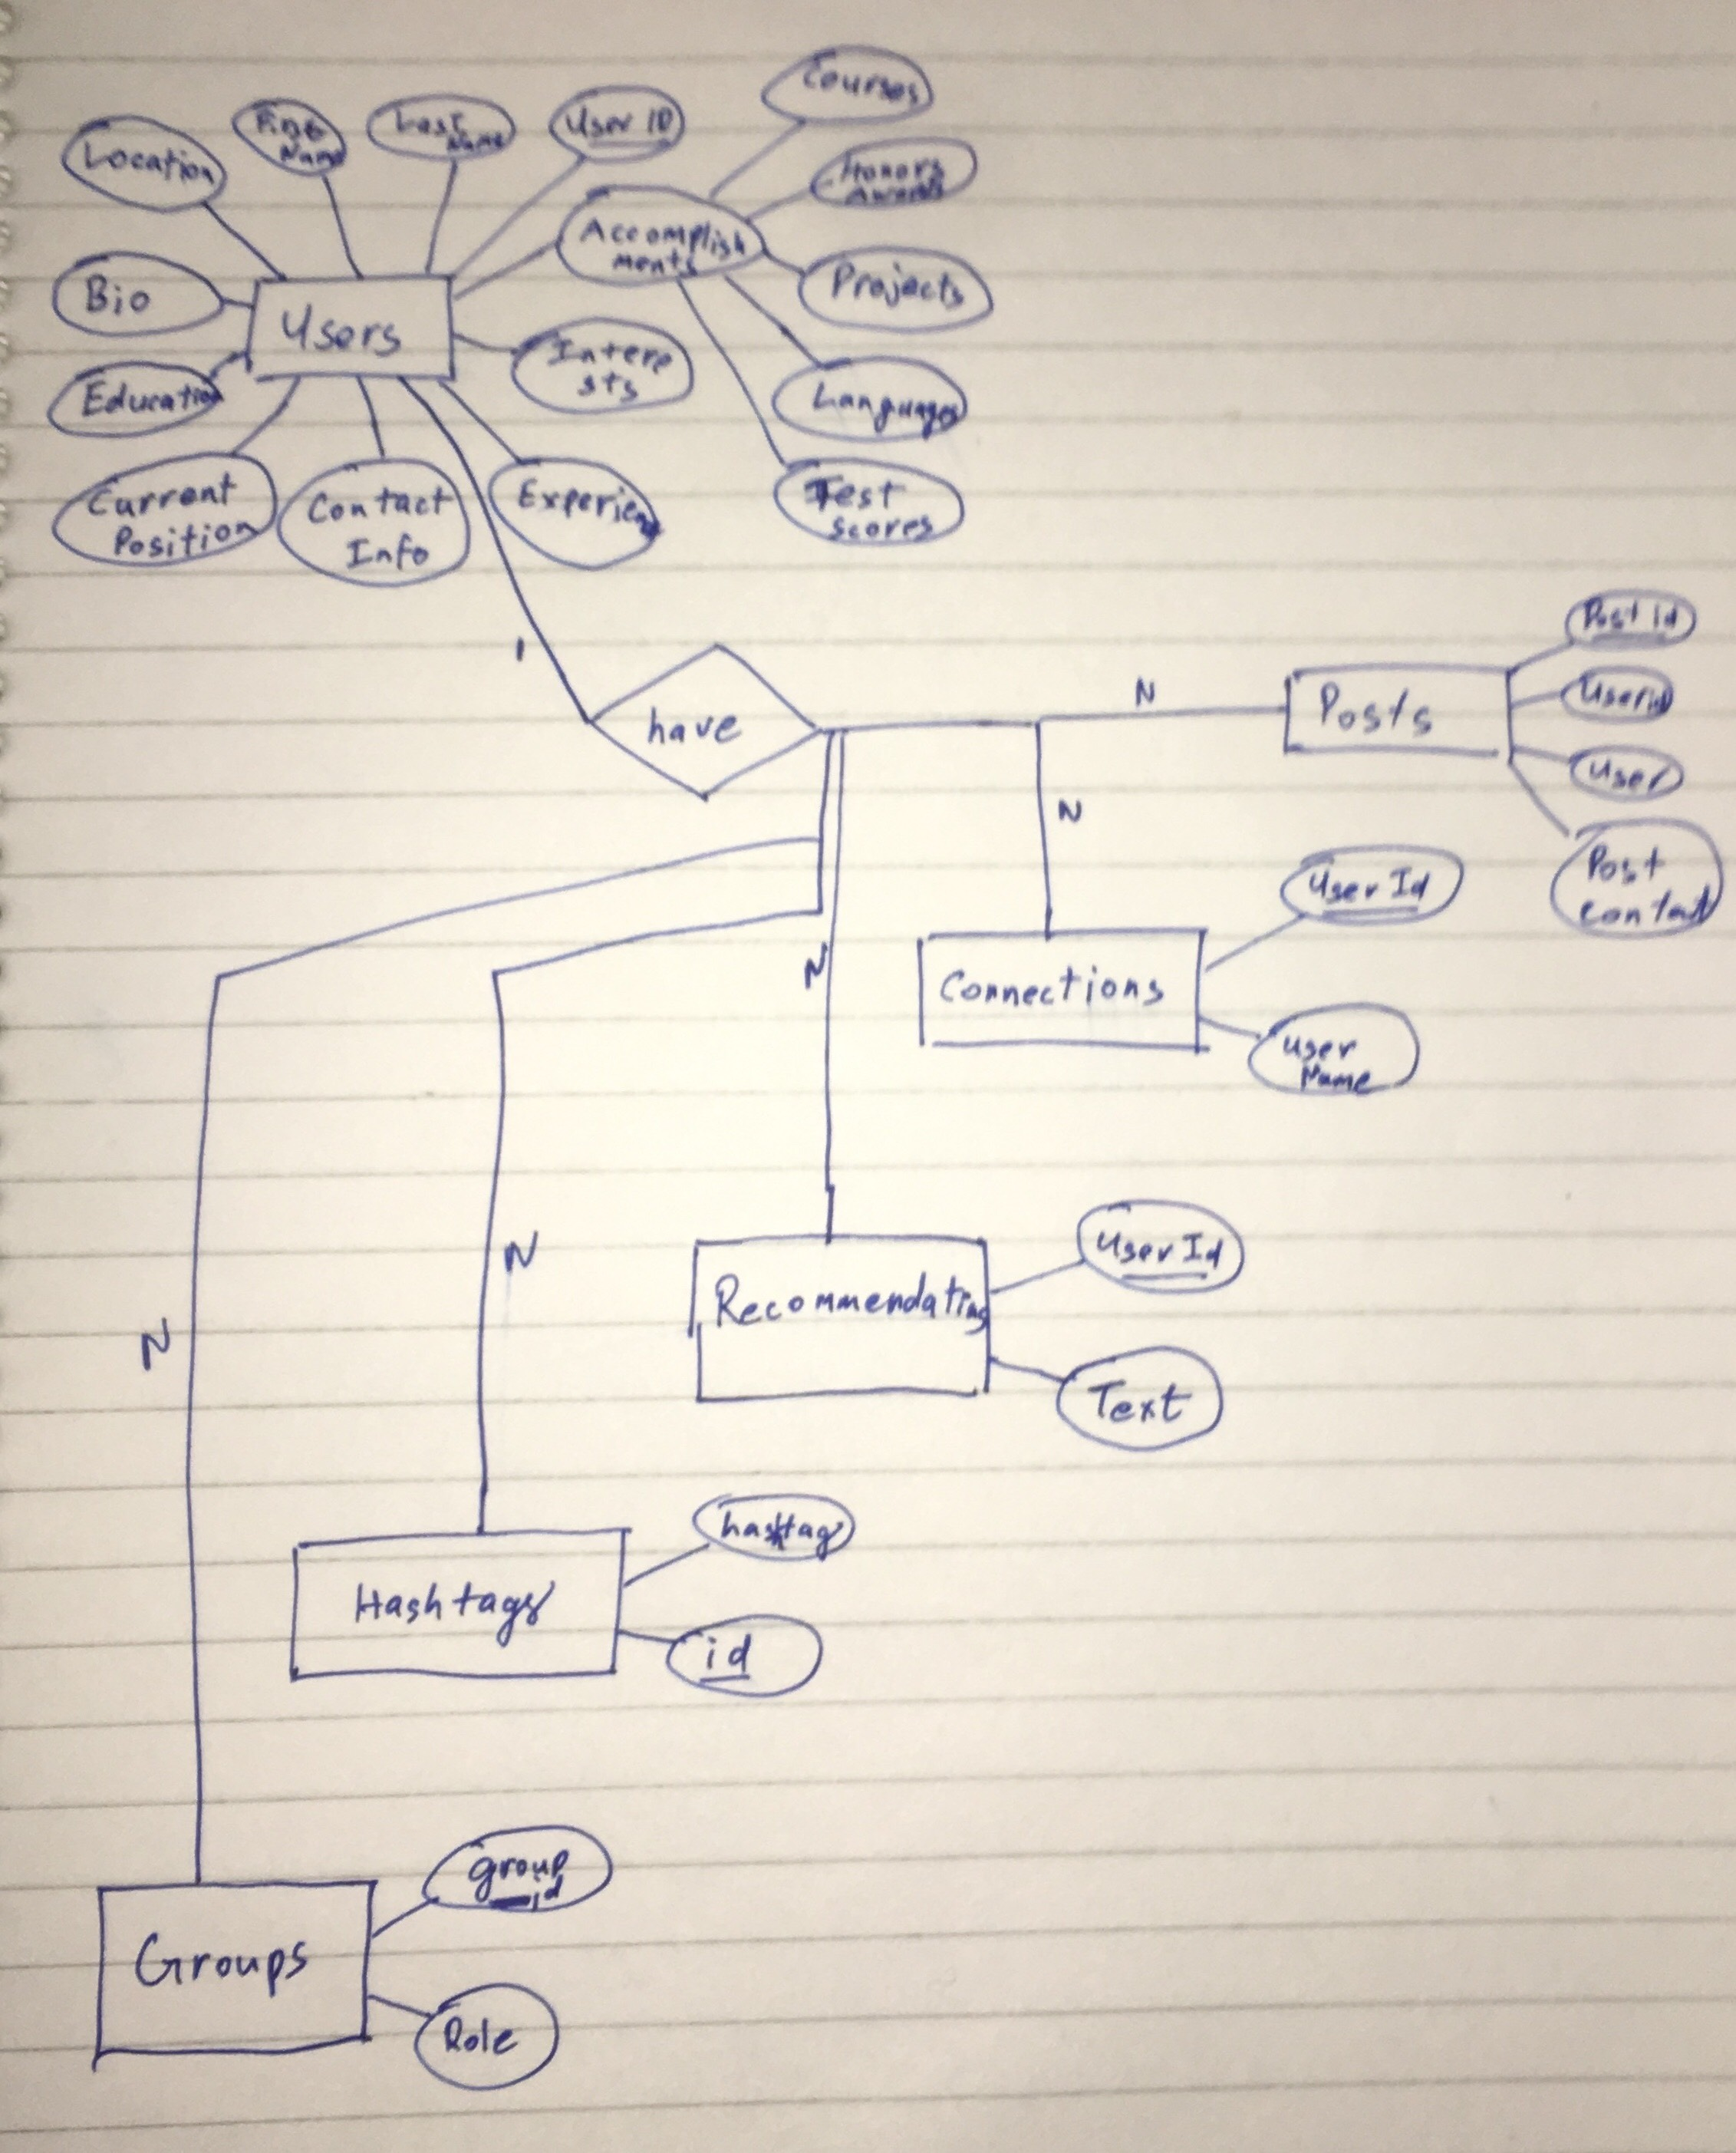
\includegraphics[width=400pt]{erdiagram.jpg}
    \caption{ER Diagram of Linkedin Site}
    \label{fig:my_label}
\end{figure}
%%% Fill in your content here.
\subsection{Set of relations}
%%% Fill in your content here.
User-Recommendation( From\_user\_id, To\_user\_id) \\
User-Connection(User\_id\_1, User\_id\_1) \\
User-post(Post\_id, User\_id) \\
User-hashtags(hashtag\_id, user\_id) \\
User-groups(group\_id, user\_id) \\
\subsection{Keys and FDs}
%%% Fill in your content here.
Keys: \\
User\_id, group\_id, hashtag\_id, recommendation\_id, connection\_id, Post\_id \\
Fd: \\
User\_id -\textgreater User\_name \\
User\_id -\textgreater Bio \\
User\_id -\textgreater Interests \\

\subsection{Sample Data}
%%% Fill in your content here.
Users\{ \\
	\{ \\
		User\_id: 1 \\
		User\_name: akshat \\
		Location: new delhi \\
		Education: btech \\
	\} \\
\}\\
\\
Connection\{ \\
	\{\\
		User\_id: 2 \\ 
		Username: shyam \\
	\} \\
\} \\
\\
Recommendation\{ \\
	\{ \\
		User\_id:3 \\ 
		Text: good \\
	\} \\
\} \\
\\
Posts\{c\\
	\{ \\
		Post\_id: 12 \\
		User\_id: 1 \\ 
		User: akshat \\
		Post\_content: hi there \\
	\} \\
\} \\
\\
Groups\{ \\
	\{ \\
		group\_id: 34 \\
		Role: admin \\
	\} \\
\} \\
\\
Hashtag\{ \\
	\{ \\ 
		hashtag: dbms \\
		hashtagid:56 \\
	\} \\
\} \\
\\
\subsection{List of various relationships}
%%% Fill in your content here.

Weak-entity Set: Connections and Recommendations are weak-entity set. \\
Non-binary: None of the relationship is non binary. \\
Hierarchial relationships: Admin with privileges is hierarchial relationship of user \\
Constraints: They are marked in the figure. \\
\section{Answer 2}
%% Fill in your content here.

\section{Answer 3}
\subsection{Schema}
%%% Fill in your content here.
\begin{center}
 \begin{tabular}{||c c c c c c||} 
 \hline
 Number & City & Gender & Age & Income & Illness \\  
 \hline\hline
 int & varchar & varchar &  int & float & varchar \\ 

 \hline
\end{tabular}
\end{center}
\subsection{Various insert modes}
%%% Fill in your content here.
\subsubsection{Bulk Load}
%%% Fill in your content here.
Bulk load with command \\
COPY toyset(Number, City, Gender, Age, Income, Illness) FROM \\ '/home/akshat/codes/col362/toy-dataset/toy\_dataset.csv'
DELIMITER ',' CSV HEADIER; \\
executed in 282.926 ms

\subsubsection{Insert statements}
%%% Fill in your content here.
Insert statements with command \\ 
time psql -f toy\_dataset.sql -d postgres \\ 
executed in 7 minute 22 seconds \\


% \subsubsection{using JDBC}
% %%% Fill in your content here.
\subsection{Statistics}
%%% Fill in your content here.
\begin{center}
 \begin{tabular}{||c c ||} 
 \hline
 Configuration & 10 gb Ram, Ubuntu 18.04 \\ 
 \hline
 Name of dataset & Toy Dataset \\ 
 \hline
 Size of dataset & 150000 \\
 \hline
 Bulk load time & 282.926 ms \\
 \hline
 Insert load time & 7 minute 22 seconds \\
 \hline
\end{tabular}
\end{center} 
Commands have been mentioned earlier

% \section{Answer 4}
% %%% Fill in your content here.

\end{document}

\